\chapter{序論}
\label{chap:introduction}

\section{背景}
\label{section:background}

本論文の読者は、オーディオの伝送と聞いて何を思い浮かべるだろうか。音楽をイヤホンやヘッドホンで聴くこと読者も多いだろう。スマートフォンやコンピュータといった再生機器に、3.5mmステレオミニプラグ(いわゆるイヤホンジャック)を接続するか、あるいはBluetoothといった無線伝送によってオーディオは伝送されている。

一般的な民生用オーディオ伝送では、インターフェイスや接続が手軽な利便性をとり、ある程度の音質劣化や遅延は許容されている。一方で、業務用オーディオの世界では妥協のない高音質の追求や、絶対に伝送される安定性が優先される。

プロのアーティストによるライブ、テレビ局やインターネットの動画配信などで用いられる業務用オーディオでは、民生向けで使われるオーディオ伝送に比べ、次にあげるような条件が要求される。

\begin{itemize}
  \item 高音質
  \item 低遅延
  \item 伝送の安定性
\end{itemize}

デジタル伝送技術は、アナログ伝送に比べ伝送経路による劣化が起こりにくくなっている。ただし、オーディオ入力と出力の最初と最後は図\ref{fig:first_and_last_need_ad_da}のように、必ずアナログとデジタルの変換(以下、A/D変換、D/A変換)が必要となる。そのため、すべての伝送経路をアナログで伝送するのに比べ、少なからず伝送するにあたりA/D変換とD/A変換にともなう遅延が発生する。しかしながら、技術の向上によって遅延量は少なくなっている。たとえば、XXXでA/D、D/A変換に要する時間はX.Xms以内である。

もう一つ、デジタル伝送を行なうことによる恩恵は高音質のまま伝送できることである。アナログ伝送のまま伝送を行えば、理論的にはA/D、D/A変換を挟まないため、劣化しないはずである。しかしながら、アナログ伝送は外部からのノイズに弱く、伝送経路中で劣化する可能性が否定できない。そこで、デジタル伝送ではアナログ信号を0と1の信号にする。

\begin{figure}[htbp]
  \centering
  \label{fig:first_and_last_need_ad_da}
  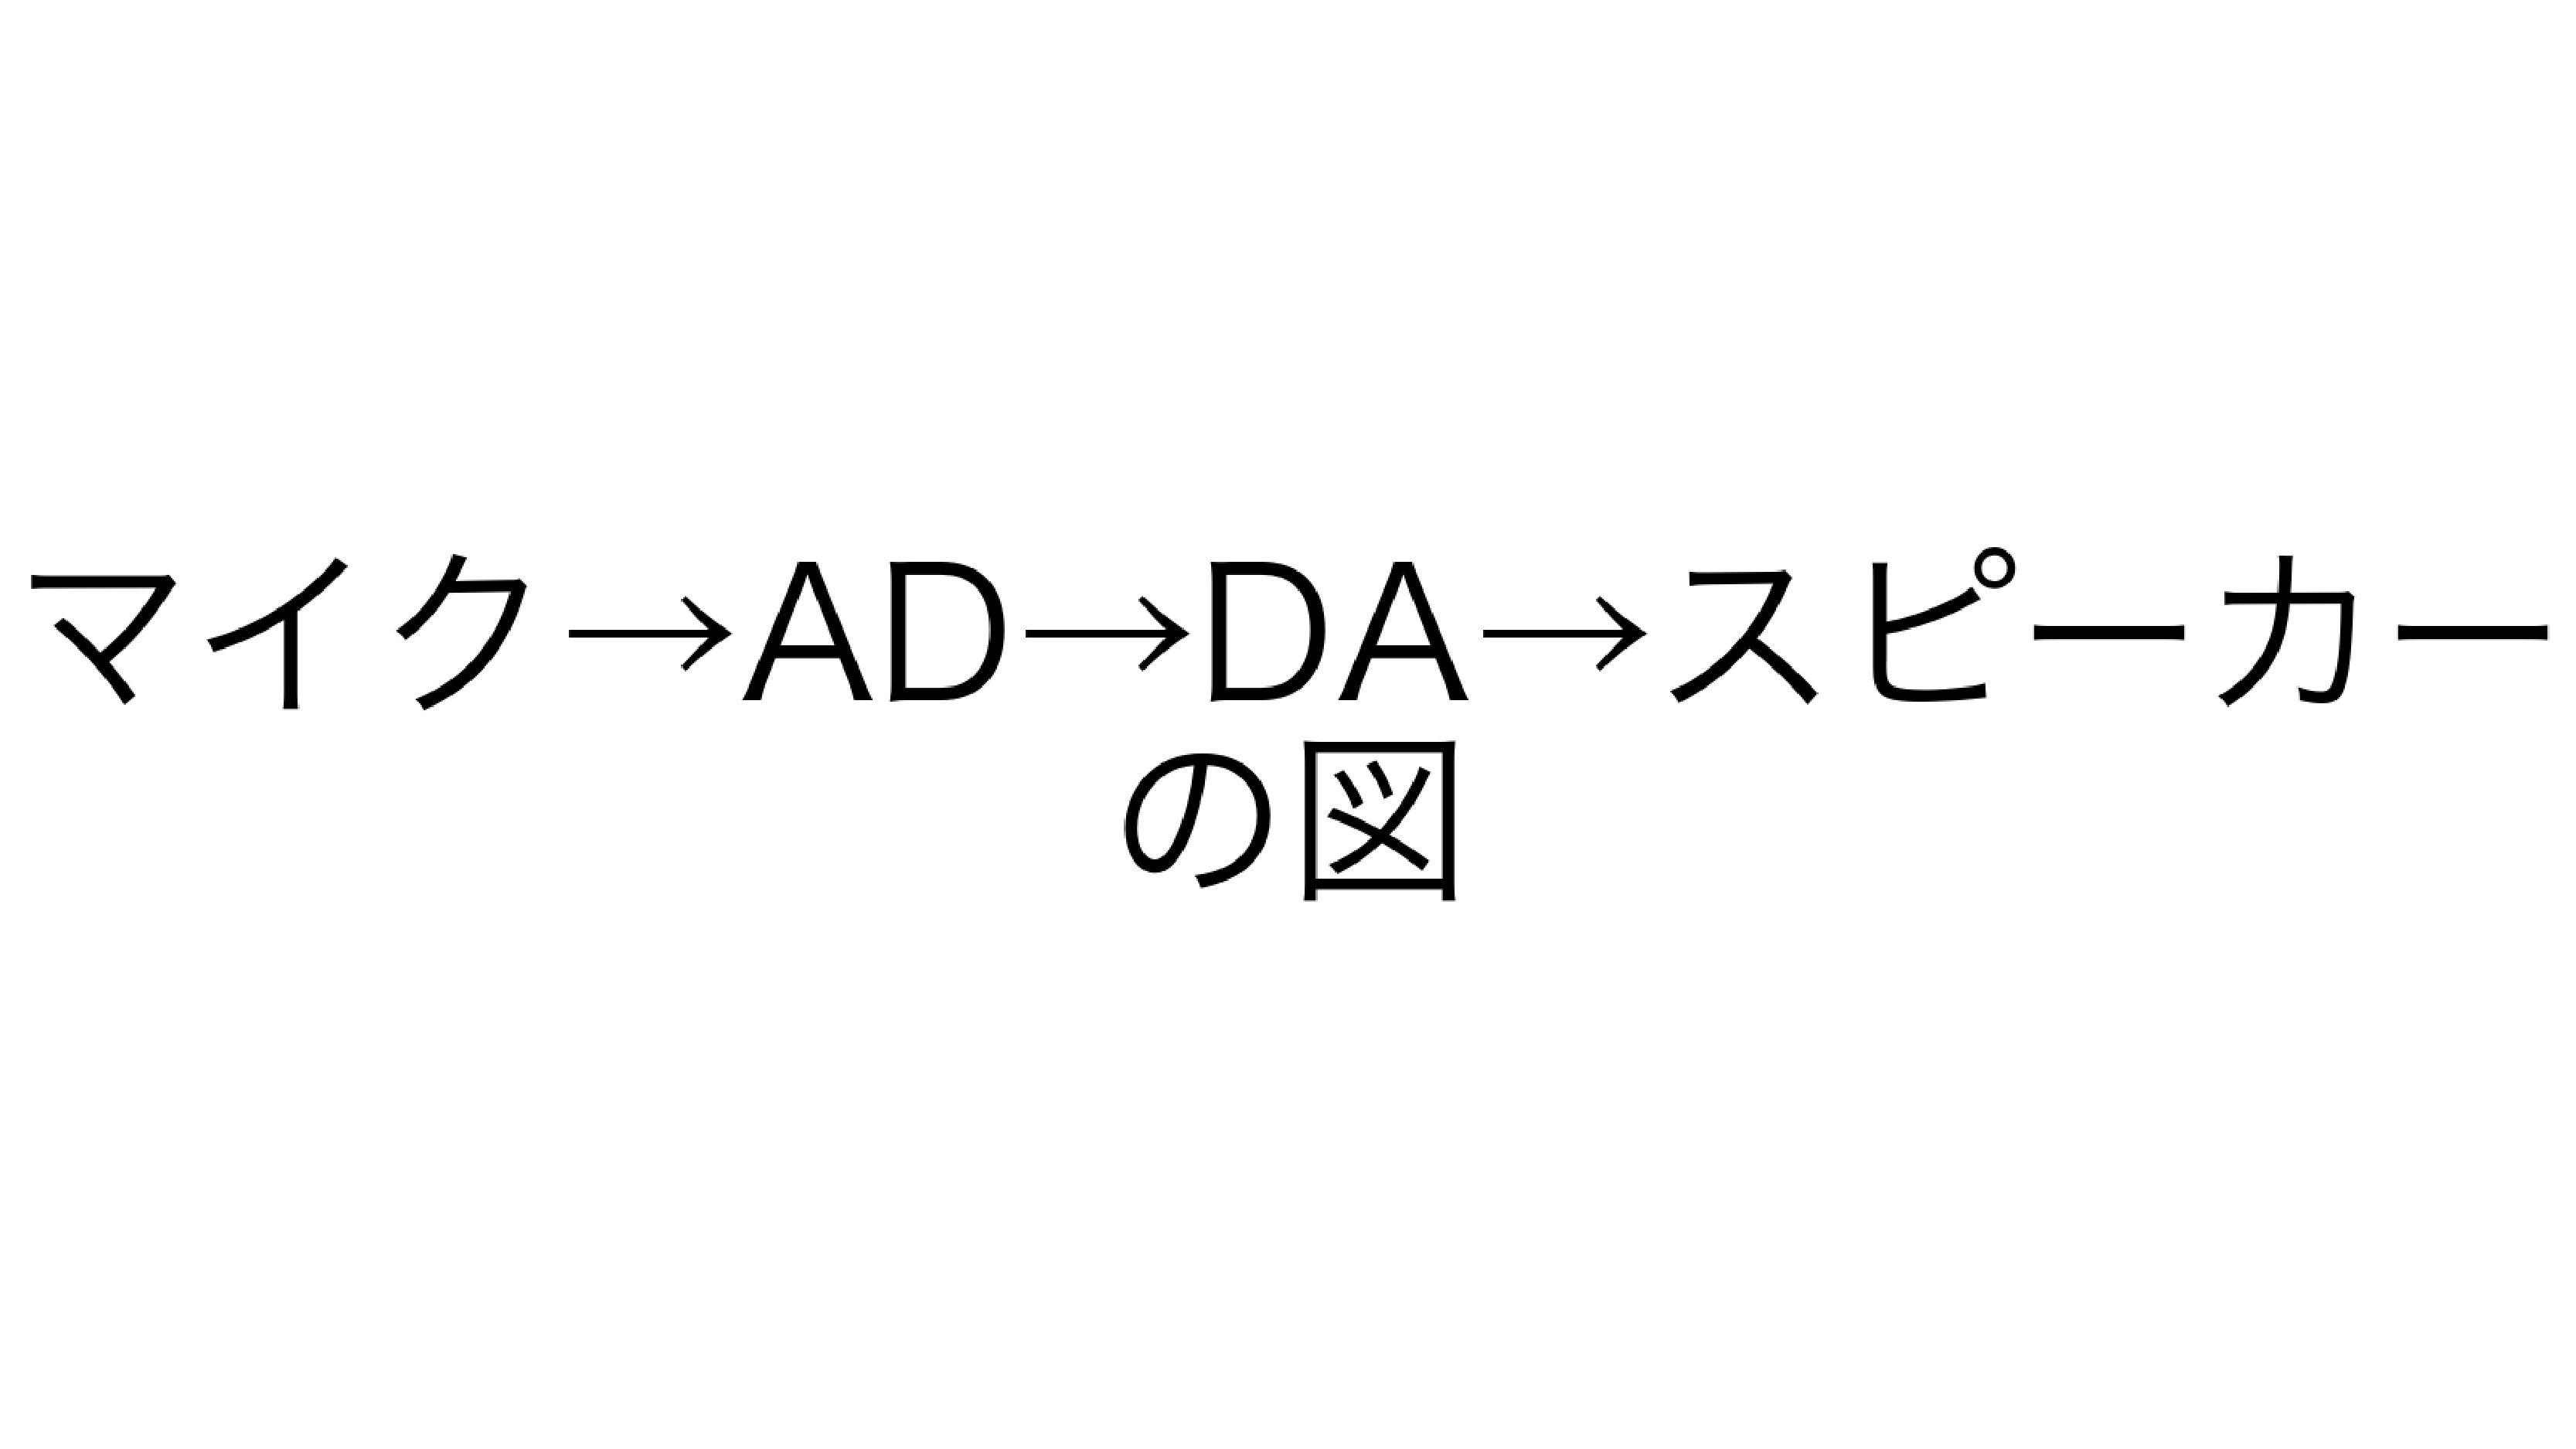
\includegraphics[width=0.8\linewidth]{img/first_and_last_need_ad_da.pdf}
  \caption{マイク→AD→DA→スピーカーの図}
\end{figure}

〜〜という理由によってIPベースの伝送への期待が高まっている。

したがって、オープンなIPベースのデジタルオーディオ伝送が必要である。

そこで、登場したのがAES67だ。AES67は、乱立する既存のIPベースのデジタルオーディオ伝送技術を共通化し、相互運用性を高めるための規格である。今後、オーディオのIP伝送が主流となっていくなかで、オープンな標準化技術によってさまざまなオーディオ機器を接続できることは重要である。

\section{本論文の目的}

前述したAES67について、オーディオストリームを送受信するアプリケーションを実装する。既存の商用規格から置き換えが可能なのか、業務用途で要求される厳しい条件に耐えられるかを検証する。

\section{本論文の構成}

本論文における以降の構成は次の通りである。

\ref{chap:related_works}章では、本論文で扱うIPベースのオーディオ伝送について理解ための前提技術について、解説する。業務用オーディオが使われている現場の構成、さらにはオーディオのデジタル伝送技術について触れる。

\ref{chap:design}章では、AES67を用いたIPベースのオーディオ伝送の送受信を行なうアプリケーションの設計を行い、その内容について述べる。

\ref{chap:implementation}章では、\ref{chap:design}章で設計したアプリケーションを実装し、その内容について述べる。

\ref{chap:evaluation}章では、\ref{chap:implementation}章で実装したアプリケーションをもとに、実際の業務用オーディオ環境を模した実験を行い、評価した結果について述べる。

\ref{chap:conclusion}章では、本研究における結論と今後の展望、業務用オーディオの伝送技術の未来について述べる。
